\documentclass[a6paper, 12pt, parskip=half, DIV=14]{scrartcl}

\usepackage{dessertdice}

\usepackage{ragged2e}
% Minimize unwanted hyphenation
\tolerance=1
\emergencystretch=\maxdimen
\hyphenpenalty=1
\hbadness=10000

\usepackage{enumitem}

\raggedright
\pagestyle{empty}
\pagecolor{black}
\begin{document}

\begin{titlepage}
\enlargethispage{3.5\baselineskip}
\setmainfont[Scale=2.75]{LondrinaSolid}
%\setmainfont[Scale=1.9]{LondrinaSolid-Black}
\Huge
\phantom{a}
\vspace{-1.75ex}
\begin{center}
%\textcolor{white}{Dessert \\[0.25ex]\tikz{\node[inner sep=0pt] {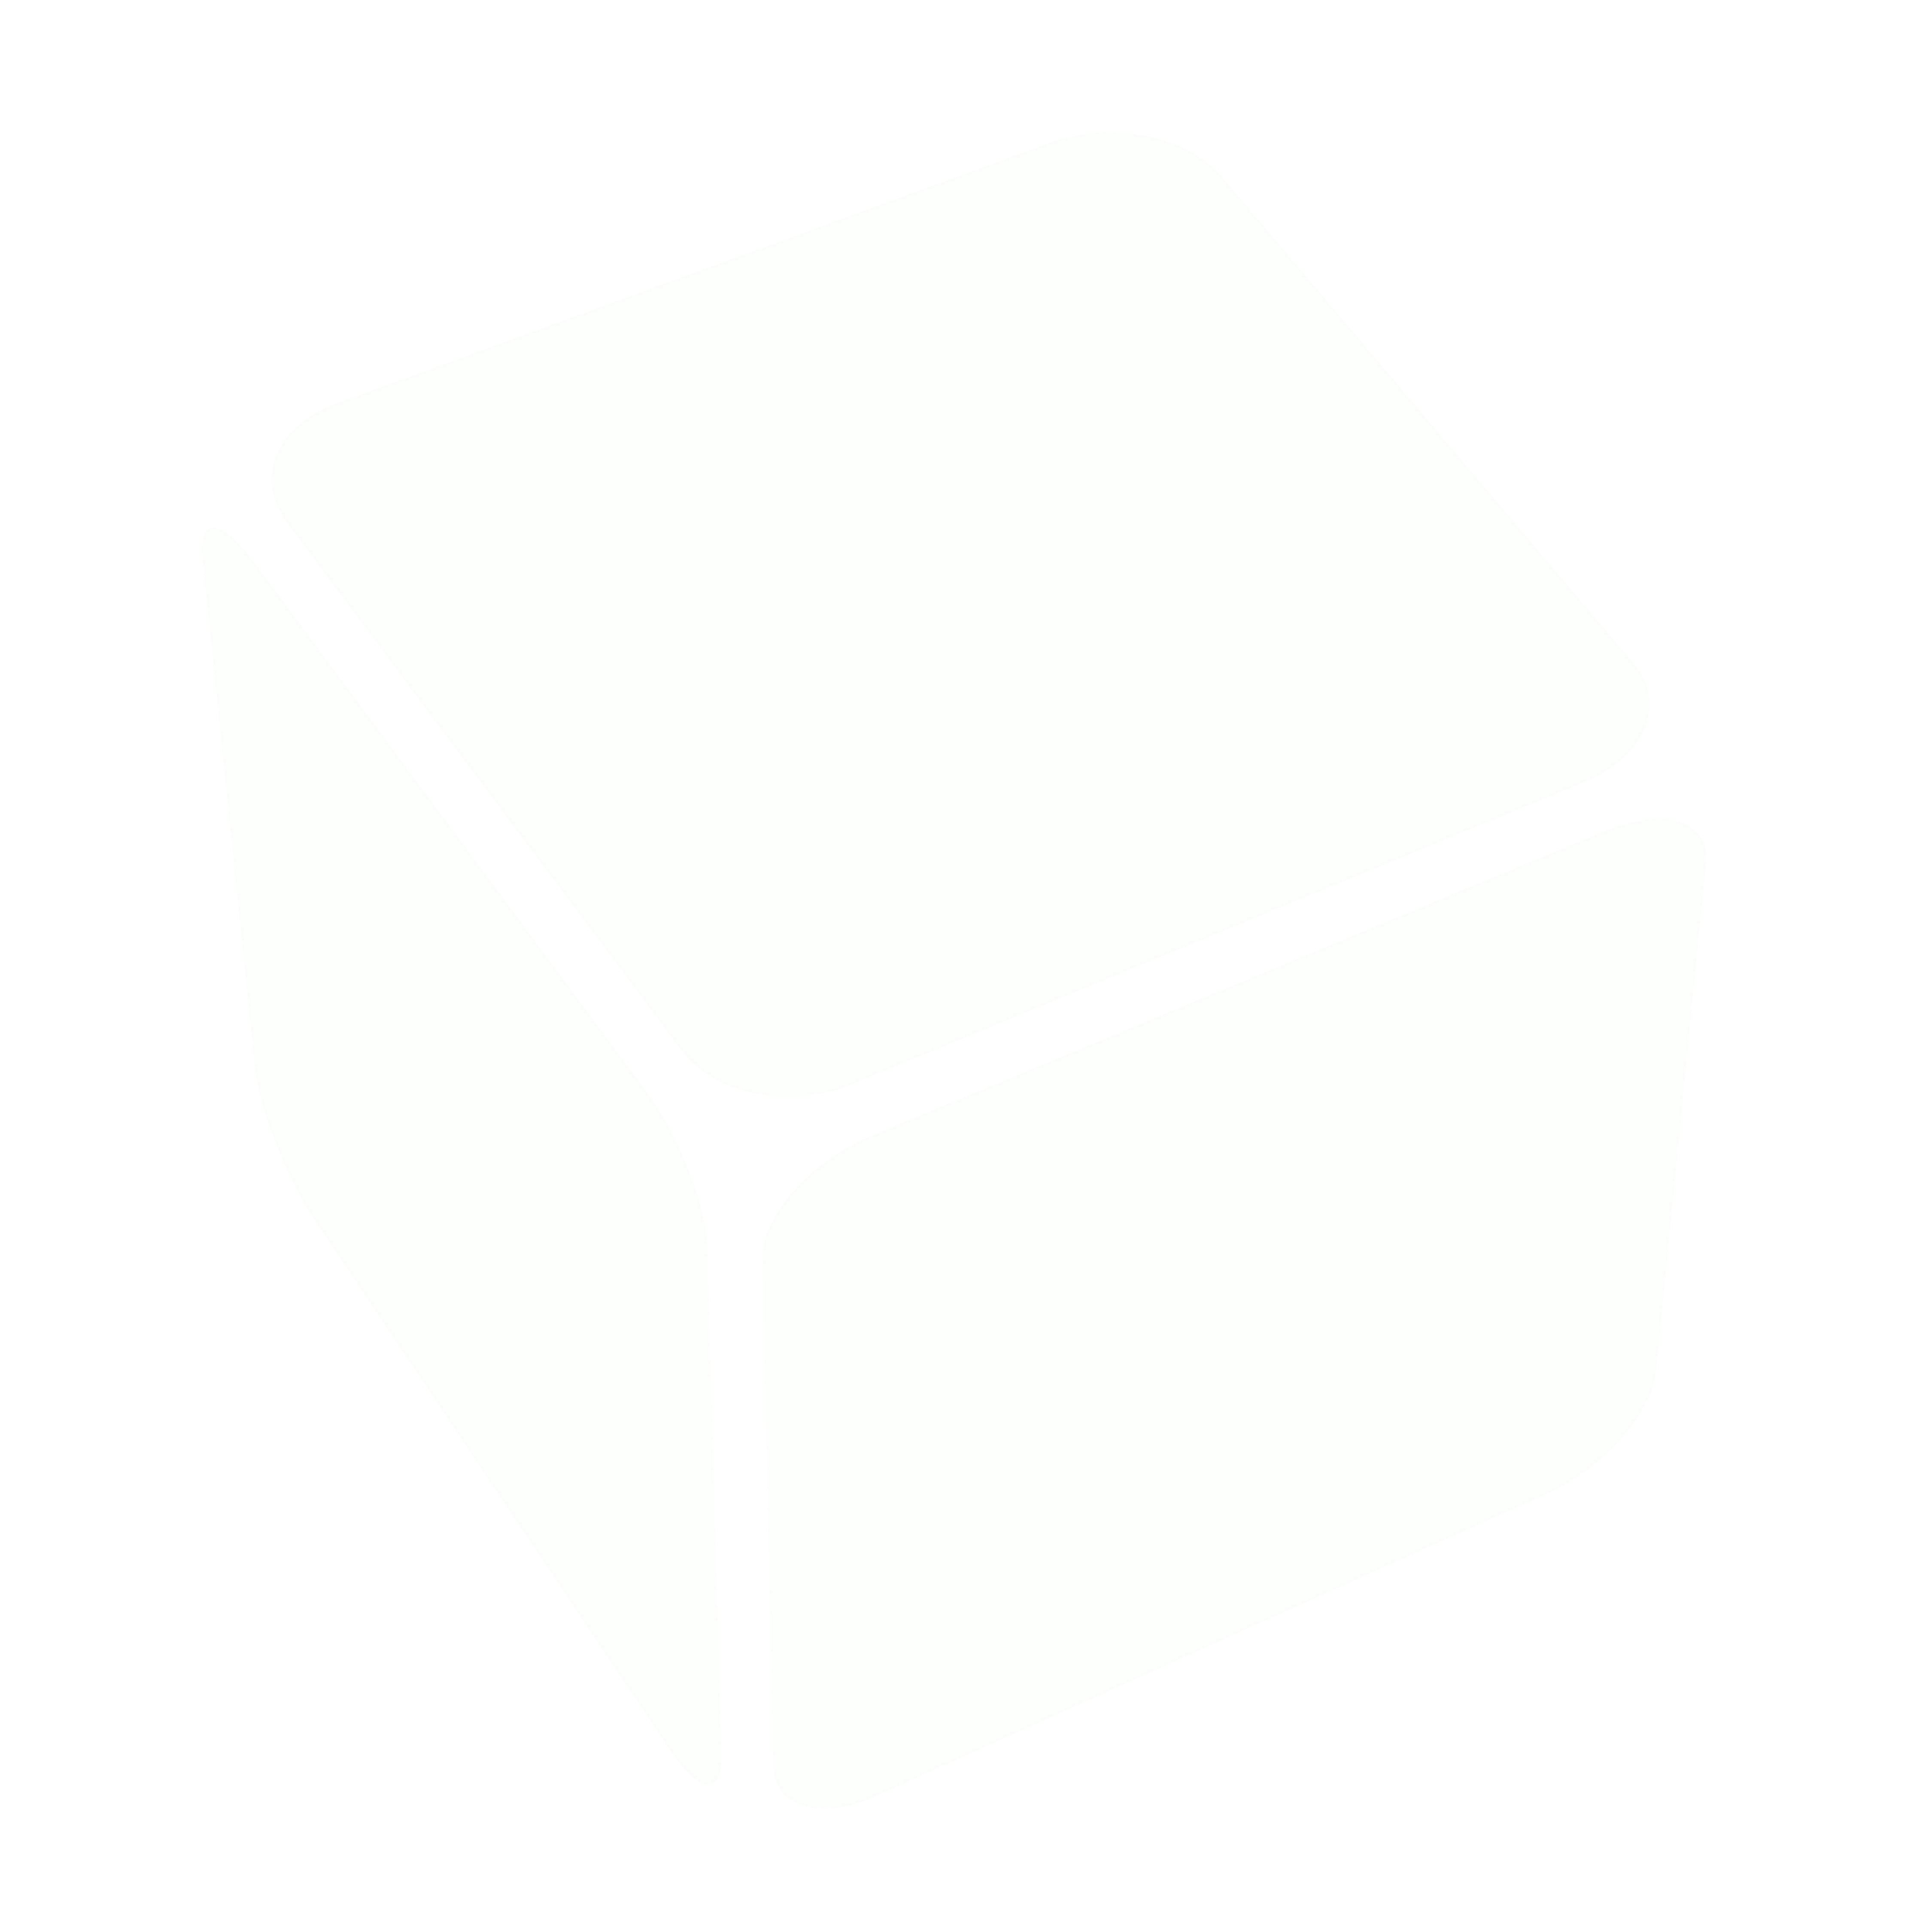
\includegraphics[height=1.375ex]{Images/blank_die3b.png}};}\hfill Dice\hfill\tikz{\node[inner sep=0pt] {
\includegraphics[height=1.375ex]{Images/blank_die2b.png}};}}
%\textcolor{white}{Dessert Dice}
\textcolor{white}{Dessert \\[0.25ex]\hspace{0.25ex}Dice \hspace{0.25ex}\tikz{\node[inner sep=0pt] {
\includegraphics[height=1.5ex]{Images/pair_of_dice.png}};}}
\end{center}

\vfill

\setmainfont[Scale=2.5]{LondrinaSolid}
\normalsize

\begin{itemize}[itemindent=0.4cm]
%\def\labelitemi{\tikz{\node[inner sep=0pt, minimum height=2.5ex, minimum width=2.5ex] {
\includegraphics[height=2.5ex]{Images/SweetsIcons/jello2.png}};}}
%	\item \ \raisebox{0.5ex}{\textcolor{JelloRed}{Jello Tart}} \hfill \raisebox{0.5ex}{\textcolor{JelloRed}{- \ \$2}}
\def\labelitemi{\tikz{\node[inner sep=0pt, minimum height=2.5ex, minimum width=2.5ex] {
\includegraphics[height=2.5ex]{Images/SweetsIcons/jello_orange2.png}};}}
	\item \ \raisebox{0.5ex}{\textcolor{JelloOrange}{Jelly Tart}} \hfill \raisebox{0.5ex}{\textcolor{JelloOrange}{- \ \$2}}
\def\labelitemi{\tikz{\node[inner sep=0pt, minimum height=2.5ex, minimum width=2.5ex] {
\includegraphics[height=2ex]{Images/SweetsIcons/jellyroll2.png}};}}
	\item \ \raisebox{0.5ex}{\textcolor{ScrollYellow}{Sweet Roll}} \hfill \raisebox{0.5ex}{\textcolor{ScrollYellow}{- \ \$2}}
\def\labelitemi{\tikz{\node[inner sep=0pt, minimum height=2.5ex, minimum width=2.5ex] {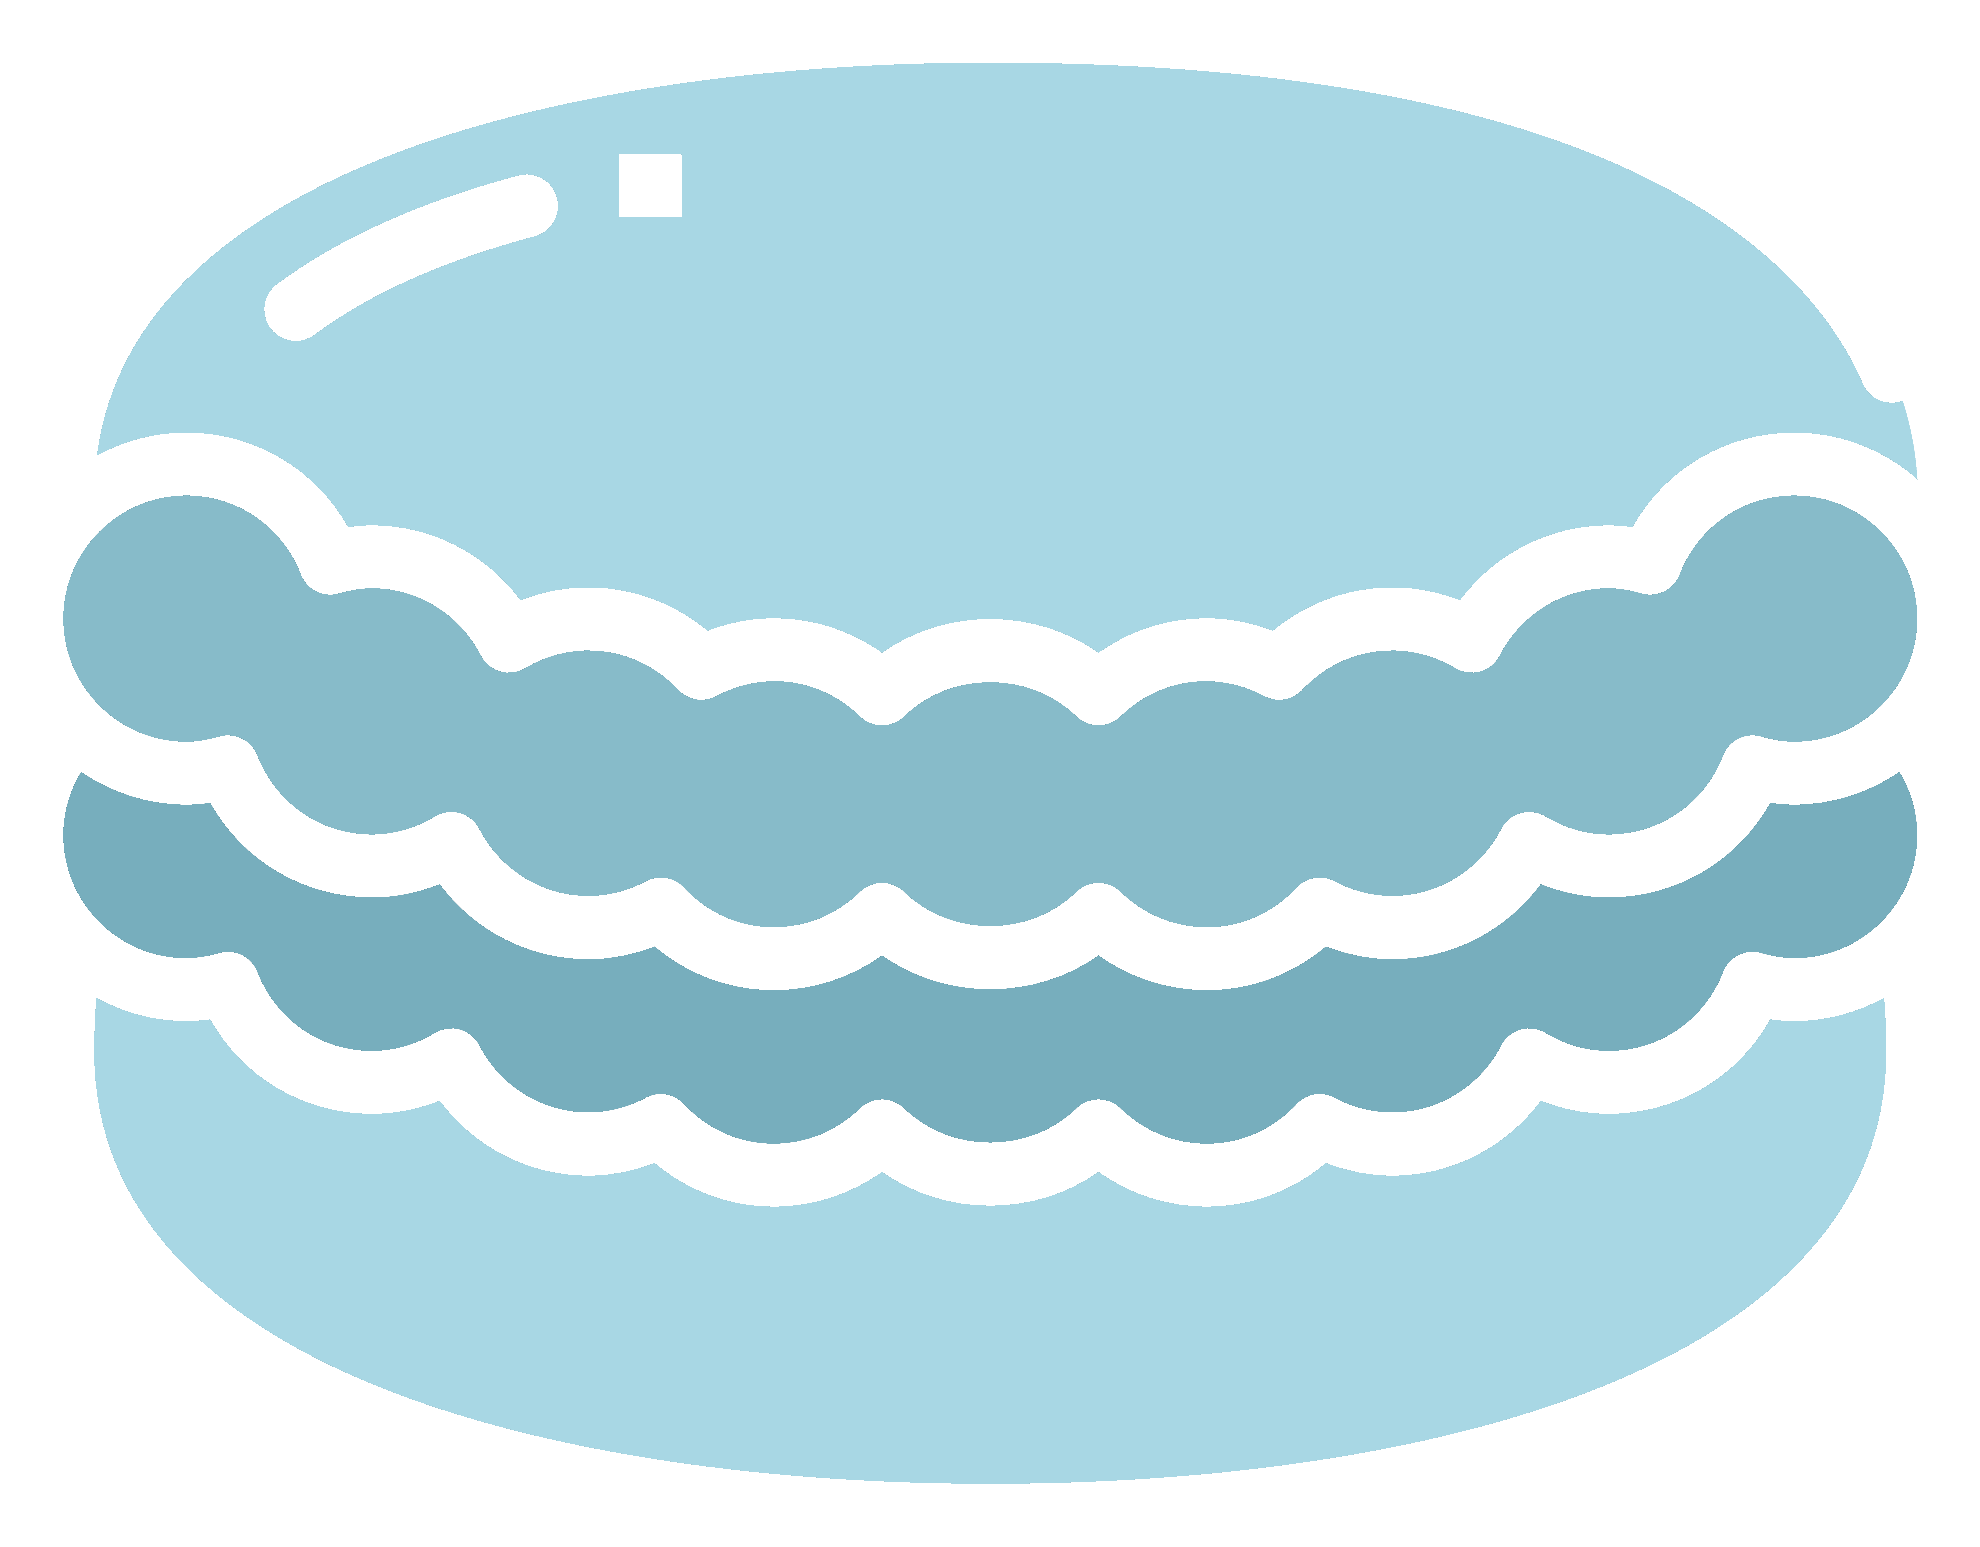
\includegraphics[height=2ex]{Images/SweetsIcons/macaron2.png}};}}
	\item \ \raisebox{0.5ex}{\textcolor{MacaronBlue}{Macaron}} \hfill \raisebox{0.5ex}{\textcolor{MacaronBlue}{- \ \$2}}
%\def\labelitemi{\tikz{\node[inner sep=0pt, minimum height=2.5ex, minimum width=2.5ex] {
\includegraphics[height=2.5ex]{Images/SweetsIcons/popsicle_green2.png}};}}
%	\item \ \raisebox{0.5ex}{\textcolor{PopsicleGreen}{Popsicle}} \hfill \raisebox{0.5ex}{\textcolor{PopsicleGreen}{- \ \$2}}
\def\labelitemi{\tikz{\node[inner sep=0pt, minimum height=2.5ex, minimum width=2.5ex] {
\includegraphics[height=2.5ex]{Images/SweetsIcons/icecream2.png}};}}
	\item \ \raisebox{0.5ex}{\textcolor{IceCreamPurple}{Ice Cream}} \hfill \raisebox{0.5ex}{\textcolor{IceCreamPurple}{- \ \$2}}

\end{itemize}

\Large
\setmainfont[Scale=1.05]{Playball}
\vfill
\begin{center}
\begin{tikzpicture}
\node[draw, white, line width=1mm, rounded corners=3mm, text width = 75mm, align=center, text height=2.25ex] at (0,0) {\textcolor{white}{Designed by Michael Purcell}};
\end{tikzpicture}
\end{center}
%\normalsize
%\phantom{a}
\end{titlepage}


\end{document}